\documentclass[twoside,a4paper]{article}
\usepackage{geometry}
\geometry{margin=1.5cm, vmargin={0pt,1cm}}
\setlength{\topmargin}{-1cm}
\setlength{\paperheight}{29.7cm}
\setlength{\textheight}{25.3cm}

% useful packages.
\usepackage{amsfonts}
\usepackage{amsmath}
\usepackage{amssymb}
\usepackage{amsthm}
\usepackage{enumerate}
\usepackage{graphicx}
\usepackage{multicol}
\usepackage{fancyhdr}
\usepackage{layout}
\usepackage{tabularx}
\usepackage{xeCJK}

% some common command
\newcommand{\dif}{\mathrm{d}}
\newcommand{\avg}[1]{\left\langle #1 \right\rangle}
\newcommand{\difFrac}[2]{\frac{\dif #1}{\dif #2}}
\newcommand{\pdfFrac}[2]{\frac{\partial #1}{\partial #2}}
\newcommand{\OFL}{\mathrm{OFL}}
\newcommand{\UFL}{\mathrm{UFL}}
\newcommand{\fl}{\mathrm{fl}}
\newcommand{\op}{\odot}
\newcommand{\Eabs}{E_{\mathrm{abs}}}
\newcommand{\Erel}{E_{\mathrm{rel}}}

\begin{document}

\pagestyle{fancy}
\fancyhead{}
\lhead{俞璐 (3180104284)}
\chead{Project2-设计文档}
\rhead{2021/06/5}

\section*{I. 整体框架的UML图}
\begin{center}
    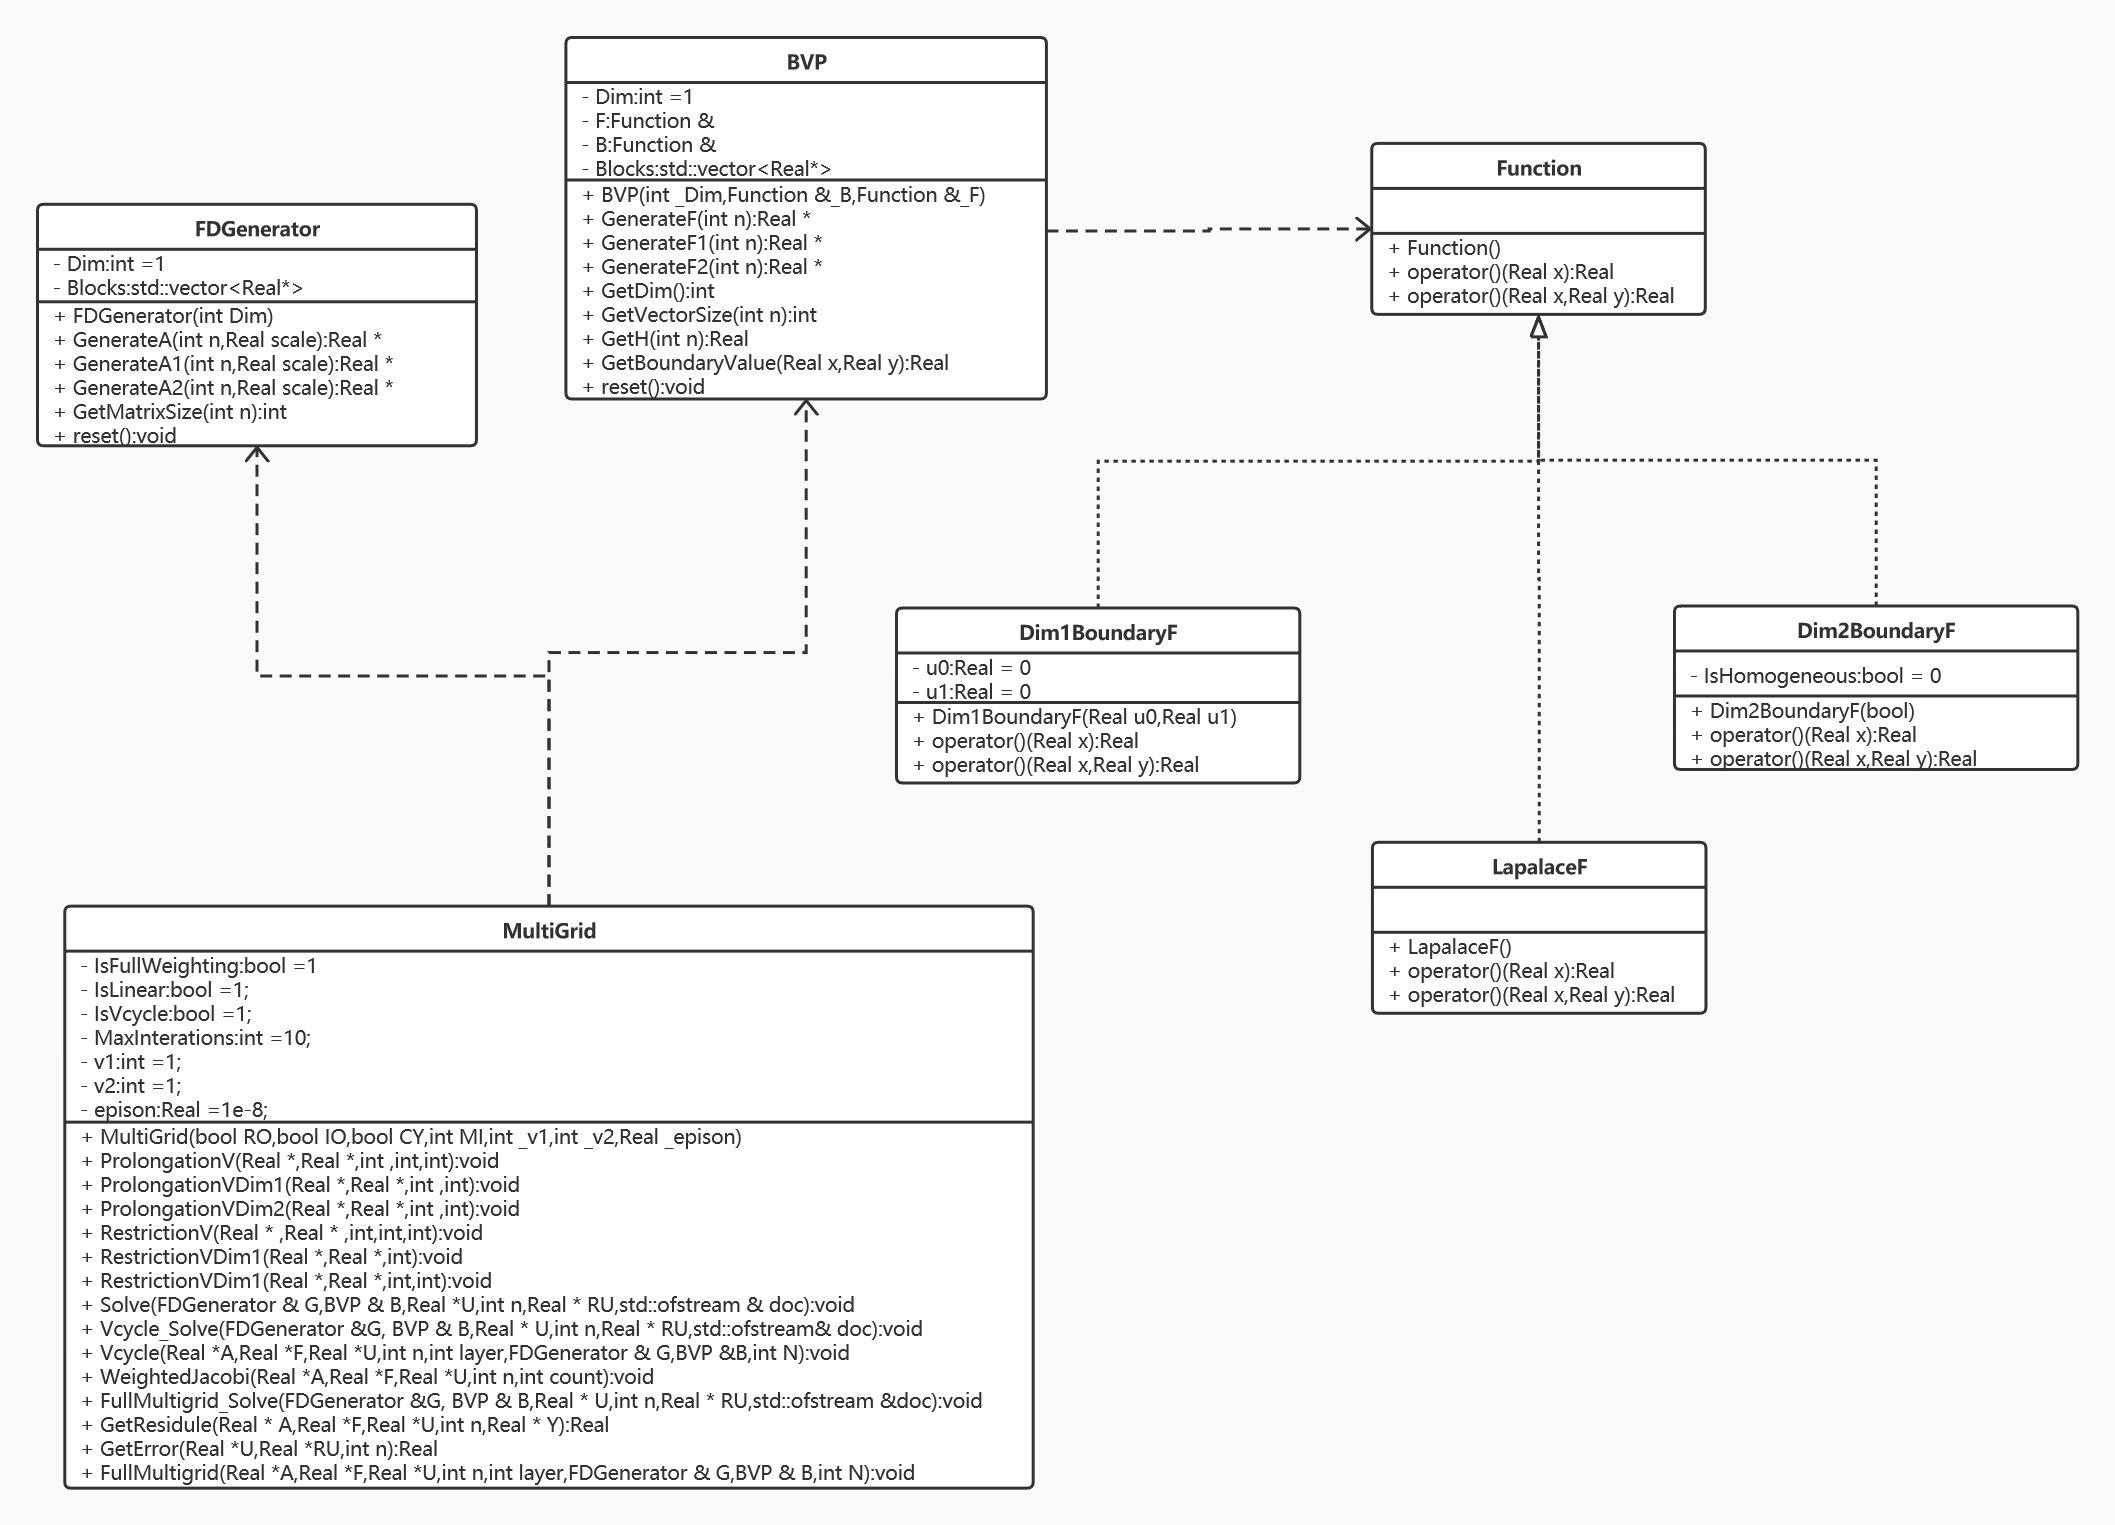
\includegraphics[scale=0.23]{../png/uml.png}
\end{center}

\section*{II. 各个类的主要组成说明}
\subsection*{II-a. 类Function}
类Function是一个对解析函数求值的虚基类,后续的边界值计算以及Lapalace算子的计算都需要继承该虚基类.
其中的主要成员函数有
\begin{center}
    \begin{tabular}{c|c}
        主要成员函数 & 具体作用                            \\
        \hline
        operator()   & 该函数可以获取一维的函数在x的取值   \\
        operator()   & 该函数可以获取二维函数在(x,y)的取值 \\
    \end{tabular}
\end{center}

\subsection*{II-b. 类Dim1BoundaryF}
类Dim1BoundaryF继承类Function,适用于一维的方程,同时增加了两个Real类型成员变量u0,u1分别表示在x=0和x=1的函数取值.

\subsection*{II-c. 类Dim2BoundaryF}
类Dim2BoundaryF继承类Function,适用于一维的方程,同时增加了一个bool类型成员变量IsHomogeneous,表示边界条件是否是齐次的.

\subsection*{II-d. 类LapalaceF}
类LapalaceF继承类Function,对应于Lapalace算子,用于求对应位置的散度.

\newpage
\subsection*{II-e. 类BVP}
类BVP对应于一个泊松方程的边值问题.
其中的主要成员变量和函数有
\begin{center}
    \begin{tabular}{c|c}
        主要成员变量 & 具体意义                                          \\
        \hline
        Dim          & 代表该边值问题的维度                              \\
        F            & 获取不同位置的散读的Function类                    \\
        B            & 获取边界处的函数值                                \\
        Blocks       & 存储在后续生成向量时产生的指针,便于最后一起delete \\
    \end{tabular}
\end{center}

\begin{center}
    \begin{tabular}{c|c}
        主要成员函数     & 具体作用                                             \\
        \hline
        GenerateF        & 根据维度来分别调用后续两个函数来产生离散系统的右端项 \\
        GenerateF1       & 根据分割的数目n来产生一维问题的右端项                \\
        GenerateF2       & 根据分割的数目n来产生二维问题的右端项                \\
        GetBoundaryValue & 通过成员变量B来计算(x,y)处的边界值                   \\
        reset            & 将Blocks所存储的Real*(所有右端项)全部delete          \\
    \end{tabular}
\end{center}

\subsection*{II-f 类FDGenerator}
类FDGenerator对应于一个生成泊松方程的离散化所对应的系数矩阵.
其中的主要成员变量和函数有
\begin{center}
    \begin{tabular}{c|c}
        主要成员变量 & 具体意义                                          \\
        \hline
        Dim          & 代表该边值问题的维度                              \\
        Blocks       & 存储在后续生成向量时产生的指针,便于最后一起delete \\
    \end{tabular}
\end{center}

\begin{center}
    \begin{tabular}{c|c}
        主要成员函数 & 具体作用                                               \\
        \hline
        GenerateA    & 根据维度来分别调用后续两个函数来产生离散系统的系数矩阵 \\
        GenerateA1   & 根据分割的数目n来产生一维问题的系数矩阵                \\
        GenerateA2   & 根据分割的数目n来产生二维问题的系数矩阵                \\
        reset        & 将Blocks所存储的Real*(所有系数矩阵)全部delete          \\
    \end{tabular}
\end{center}

\subsection*{II-g 类MultiGrid}
类MultiGrid对应于多重网格的求解器.
其中的主要成员变量和函数有
\begin{center}
    \begin{tabular}{c|c}
        主要成员变量    & 具体意义                                           \\
        \hline
        IsFullWeighting & 判断是否使用full-weighting,False则直接保留对应位置 \\
        IsLinear        & 判断是否使用线性插值,False则使用二次插值           \\
        IsVcycle        & 判断是否使用V-cycle,False则使用FMG                 \\
        MaxInterations  & 最大迭代次数                                       \\
        v1              & V-cycle中的$v_1$                                   \\
        v2              & V-cycle中的$v_2 $                                  \\
        epison          & 相对误差的终止条件                                 \\
    \end{tabular}
\end{center}

\begin{center}
    \begin{tabular}{c|c}
        主要成员函数         & 具体作用                                             \\
        \hline
        ProlongationV        & 根据维度来分别调用后续两个函数来实现Prolongation算子 \\
        ProlongationVDim1    & 实现维度为一的Prolongation算子                       \\
        ProlongationVDim2    & 实现维度为二的Prolongation算子                       \\
        RestrictionV         & 根据维度来分别调用后续两个函数来实现Restriction算子  \\
        RestrictionVDim1     & 实现维度为一的Restriction算子                        \\
        RestrictionVDim2     & 实现维度为二的Restriction算子                        \\
        Solve                & 根据IsVcycle来选择不同的求解算法                     \\
        Vcycle\_Solve        & 使用V-cycle求解                                      \\
        Vcycle               & 一次V-cycle迭代                                      \\
        WeightedJacobi       & 带权重的Jacobi迭代                                   \\
        FullMultigrid\_Solve & 使用FMG求解                                          \\
        FullMultigrid        & 一次FMG求解                                          \\
        GetResidule          & 获取残差                                             \\
        GetError             & 获取误差                                             \\
    \end{tabular}
\end{center}

\end{document}

%%% Local Variables: 
%%% mode: latex
%%% TeX-master: t
%%% End: 

